%
% main.tex -- Paper zum Thema <antennen>
%
% (c) 2020 Autor, OST Ostschweizer Fachhochschule
%
% !TEX root = ../../buch.tex
% !TEX encoding = UTF-8
%
\chapter{Antennen\label{chapter:antennen}}
\kopflinks{Antennen}
\begin{refsection}
\chapterauthor{Baris Catan und Jannis Gull}
\index{Baris Catan}%
\index{Catan, Baris}%
\index{Jannis Gull}%
\index{Gull, Jannis}%

\noindent
Das Ziel dieses Kapitels ist, den Wirkungsgrad einer dreieckigen Loop-Antenne mittels 
\index{Loop-Antenne}%
Formoptimierung zu erhöhen. Für die Umsetzung dieser Problemstellung wird 
\index{Formoptimierung}%
eine direkte Methode der Variation, in diesem Fall das Verfahren nach Ritz, 
\index{Verfahren nach Ritz}%
verwendet.

%
% antennenAllgemein.tex 
%
% 
%
% !TEX root = ../../buch.tex
% !TEX encoding = UTF-8
%

\section{Antennen\label{antennen:antennenAllgemein}}
\rhead{Antennen}

Antennen sind in der heutigen technologisch geprägten Welt nicht mehr weg zu denken. Sie befinden sich in vielen alltäglichen elektronischen Geräten. Eine Antenne wandelt die in einer Leitung geführte gebundene elektromagnetische Welle in eine freie Welle im Raum um. Da eine Antenne freie Wellen ebenso in gebundene leitungsgeführte Wellen umwandeln kann hat sie reziproke Eigenschaften.

Eine genauere Erklärung von elektromagnetischen Wechselwirkungen kann sich im \href{chapter:maxwell}{Kapitel Maxwell}, welches sich mit den Maxwell Gleichungen befasst, angeeignet werden. 
\subsection{Loop-Antennen\label{antennen:antennenAllgemein_loop}}
\rhead{Loop-Antennen}
Eine Loop-Antenne hat eine simple Funktionsweise. Sie besteht aus einem geschlossenen Stück Draht wie in Abbildung... gesehen werden kann. Die Loop-Antenne kann, nicht wie der Name impliziert, verschiedenste Formen annehmen. Durch den Leiter wird ein Signal geführt, welches in der aufgespannten Fläche ein magnetisches Feld induziert. Dieses Feld wird durch Anpassung der Signalamplitude verändert. Eine solche Änderung kann als Information angesehen werden, welche sich nun im Äter, also dem freien Raum, fortbewegt.

\subsection{Eigenschaften\label{antennen:antennenEigenschaften}}
\rhead{Eigenschaften}
Der Wirkungsgrad $\eta$ , auch Effizienz genannt, kann mittels der Gesamtleistung der Antenne P\textsubscript{tot} und der abgestrahlten Leistung P\textsubscript{rad} berechnet werden.
\section{Anfang\label{antennen:antennenAllgemein2}}
\rhead{Anfang}

hallo
%
% problemstellung.tex 
%
% 
%
% !TEX root = ../../buch.tex
% !TEX encoding = UTF-8
%

\section{Problem\label{antennen:problemstellung}}
\rhead{Problem}
 Es wird versucht eine Antenne zu designen, welche in einem Gerät mit der Form eines Prismas mit Deckfläche eines gleichseitigen Dreiecks. Dies bedeutet, dass die Antenne die Maas eines gleichseitigen Dreiecks nicht überschreiten darf.
\subsection{Geometrie\label{antennen:Geom}}
\rhead{Geometrie}
Das Ziel ist nun, den Wirkungsgrad durch Formoptimierung zu erhöhen. Die Faktoren k\textsubscript{1} und k\textsubscript{2} sind Konstanten, was bedeutet, dass für eine Erhöhung des Wirkungsgrads (Formel referenzieren oder neu Einfügen) nur die Länge l und die Fläche A veränderbar sind. In einem nächsten Schritt wird das Verhältnis
\begin{equation}
	\frac{l}{A^2}
	\label{antennen:Verhältnis}
\end{equation}
erhöht. Diese Formel muss nun auf eine implizite Funktion angewendet werden. Eine erste Idee besteht darin, die Ecken abzuflachen, da in den Ecken mit viel zusätzlicher Länge nur wenig Fläche gewonnen wird. Zuerst muss eine Funktion f(x,y) gefunden werden, welche die Ecken, wie in Abbildung... zu sehen, möglichst effizient abflacht. Danach muss bestimmt werden, in welcher Grössenordnung diese Funktion auf das Dreieck "angewendet" wird. Dies wird in Abbildung... veranschaulicht.
%
% unserRitz.tex 
%
% 
%
% !TEX root = ../../buch.tex
% !TEX encoding = UTF-8
%

\section{Ritz Verfahren Grundsätzlich\label{antennen:ritzGrundsätzlich}}

Wie schon sehr oft in diesem Buch erwähnt, gibt es das Problem, dass man für ein Funktional
\begin{equation}
I(y)=\int_{x_1}^{x_2}L(x,y(x),y'(x))\,dx
\label{antennen:normalesFunktional}
\end{equation}
eine Funktion $y(x)$ finden muss, welche das Funktional extremal macht.
Solch eine Funktion ist die Lösung der
\begin{equation}
\frac{\partial L}{\partial y} - \frac{d}{dx} \left( \frac{\partial L}{\partial y'} \right) = 0
\label{antennen:el-DGL}
\end{equation}
Euler-Lagrange Differentialgleichung.

Wenn diese Gleichung \eqref{antennen:el-DGL} jedoch analytisch unlösbar ist kommt das Verfahren nach Ritz ins Spiel.

\subsection{Approximations-Funktion nach Ritz\label{antennen:approxFunkt}}

Eine kleine Erinnerung der Fourier-Theorie, aus dieser weiss man dass periodische Funktionen $f(t)$ als Linearkombination von anderen Funktionen, im Sinne der Fourierreihe als
\begin{equation}
F R[f(t)]=\frac{a_0}{2}+\sum_{n=1}^{\infty}\left[a_n \cdot \cos \left(n \omega_f t\right)+b_n \cdot \sin \left(n \omega_f t\right)\right]
\label{antenne:fourier}
\end{equation}
beschrieben werden können.

Eine ähnliche Idee wird beim Verfahren nach Ritz angewendet.
Es wird eine approximations-Funktion in der Form
\begin{equation}
y(x)=\sum_{k=1}^n a_k \psi_k(x)
\end{equation}

definiert. Diese hat die Funktionen $\psi_k(x)$ und Koeffizienten $a_k$. 
In der Welt des Verfahrens nach Ritz heissen die Funktionen \em Koordinatenfunktionen \em und die Koeffizienten \em Koordinaten \em.

\subsection{Mögliche Approximations-Funktionen\label{antennen:approxBsp}}

Je nach Problemstellung gibt es bessere oder schlechtere approximations-Funktionen. Mögliche ausgeschriebene Funktionen können so aussehen:

\begin{equation}
	\begin{aligned}
		\text{Exponential-Entwicklung: }
		y(x)&=
		a_0+a_1 x+a_2 x^2+\cdots+a_n x^n \\
		\text{Fourier-Entwicklung: } 
		y(x)&=
		a_0+a_1\cos(x)+b_1\sin(x)+\cdots+a_n\cos(n x)+b_n\sin(n x)\\
		\text{Hyperbolische-Entwicklung: } 
		y(x)&=
		a_1 e^{\lambda x}+a_2 e^{-\lambda x}+\cdots+a_n e^{(-1)^n \lambda}
	\end{aligned}
\end{equation}

Das Ziel ist es schlussendlich das Problem so genau wie nötig mit so wenig wie möglich Koeffizienten auszudrücken.


\subsection{Unsere Approxiamtions-Funtion}








%
% ritzAufProblem.tex 
%
% 
%
% !TEX root = ../../buch.tex
% !TEX encoding = UTF-8
%



\section{Ritz Verfahren angewandt\label{antennen:ritzAnw}}

Da wird dank der Symmetrie unseres Problems geschickt das Problem auf
nur eine Ecke lokalisieren konnten, können wir das Problem nun 
ganz geschickt auf ein Koordinatensystem platzieren.

%TODO bild ist weit weg [htbp] ILLEGAL
\begin{figure}[htbp]
	\centering
	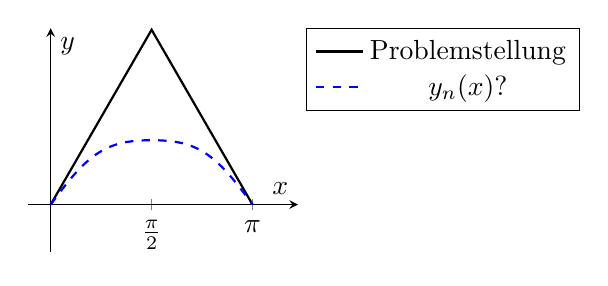
\begin{tikzpicture}
		\begin{axis}[
			scale=0.5,
			axis lines=middle,
			xlabel={$x$},
			ylabel={$y$},
			xtick={0, 1.5708, 3.14159},
			xticklabels={0, $\frac{\pi}{2}$, $\pi$},
			ytick=\empty,
			enlargelimits,
			clip=false,
			xmin=0, xmax=3.5,
			ymin=0, ymax=2,
			domain=0:pi, 
			samples=100,
			legend pos=outer north east,
			axis equal
			]
			% 3eck spitze
			\addplot[thick] coordinates {(0,0) (1.5708, pi*1.732/2) (3.14159, 0)};
			\addlegendentry{Problemstellung}
			
			\addplot[thick, blue, dashed, domain=0:3.14159, samples=100] {1.0882345*sin(deg(x))+0.0866761*sin(3*deg(x))};
			\addlegendentry{$y_n(x)?$}
		\end{axis}
	\end{tikzpicture}
	\caption{Problemstellung im Koordinatensystem}
	\label{antenenn:koordSysBsp}
\end{figure}
Um die Effizienz $\eta$ zu optimieren, müssen wir, wie in REF %~\ref{an} 
erwähnt, die quadrierte Fläche $A^2$ maximieren und die Länge $l$ für $y_n(x)$ minimieren.


\subsection{Nebenbedingungen von $y_n(x)$\label{antenennen:nebenbedRitz}}

Eine Nebenbedingung ist es, dass bei $y_n(0)$ und $y_n(\pi)$ die Funktion null sein muss.
Diese Nebenbedingung ist sehr wichtig für die Stetigkeit der finalen Form die wir optimieren.

Die Sinus-Fourier Reihe aus \eqref{antennen:unserRitz} hat eine weitere gute Eigenschaft, 
welche klar wird, wenn man in das gleiche Koordinatensystem wie bei der Abbildung \ref{antenenn:koordSysBsp}
benützt und $y_n(x)$ mit beispielsweise den Koeffizienten $a_1=a_2=1$ plottet.

%TODO bild ist weit weg [htbp] ILLEGAL
\begin{figure}[htbp]
	\centering
	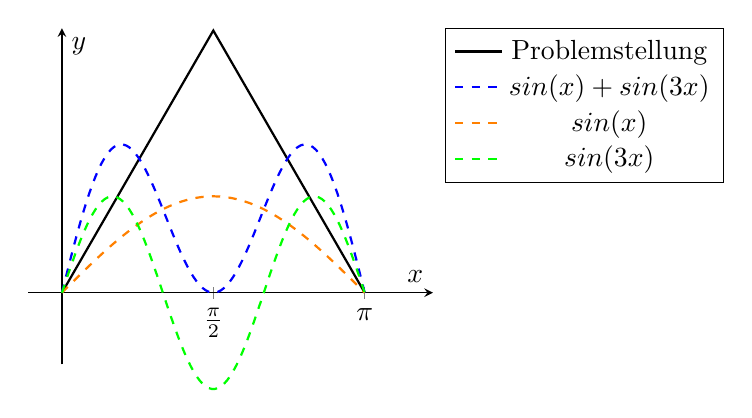
\begin{tikzpicture}
		\begin{axis}[
			scale=0.75,
			axis lines=middle,
			xlabel={$x$},
			ylabel={$y$},
			xtick={0, 1.5708, 3.14159},
			xticklabels={0, $\frac{\pi}{2}$, $\pi$},
			ytick=\empty,
			enlargelimits,
			clip=false,
			xmin=0, xmax=3.5,
			ymin=0, ymax=2,
			domain=0:pi, 
			samples=100,
			legend pos=outer north east,
			axis equal
			]
			% 3eck spitze
			\addplot[thick] coordinates {(0,0) (1.5708, pi*1.732/2) (3.14159, 0)};
			\addlegendentry{Problemstellung}
			
			\addplot[thick, blue, dashed, domain=0:3.14159, samples=100] {sin(deg(x))+sin(3*deg(x))};
			\addlegendentry{$sin(x)+sin(3x)$}
			
			\addplot[thick, orange, dashed, domain=0:3.14159, samples=100] {sin(deg(x))};
			\addlegendentry{$sin(x)$}
			
			\addplot[thick, green, dashed, domain=0:3.14159, samples=100] {sin(3*deg(x))};
			\addlegendentry{$sin(3x)$}
		\end{axis}
	\end{tikzpicture}
	\caption{Nebenbedingungen im Koordinatensystem}
	\label{fig:triangle-pgfplots}
\end{figure}

Dank der Punktsymmetrie der ungeraden Sinus-Funktionen, sind die Nebenbedingungen
\begin{equation}
	\begin{aligned}
		y_n(0)
		&=
		0
		\\
		y_n(\pi)
		&=
		0
	\end{aligned}
\label{antennen:nebenbed3eck}
\end{equation}
\em immer \em alles \em erfüllt \em zu betrachten. Im weiteren Verlaufen werden diese Nebenbedingungen somit
nicht mehr beachtet.

\subsection{NAME \label{antennen:konkreteRechnung}}

Die beste Fläche ist auch gerade die beste Fläche im quadrat \qed





%
% resultat.tex 
%
% 
%
% !TEX root = ../../buch.tex
% !TEX encoding = UTF-8
%
\usetikzlibrary{spy}
\section{Finale Überlegung\label{antennen:resultat}}

Das Kapitel \ref{antennen:ritzAnw} hat gezeigt, dass ein Abrundung an den Ecken
zur besten Effizienz führt, weil die abgerundete Form das Verhältnis \eqref{antennen:Verhältnis}
minimiert und somit die Effizienz maximiert. Wie gross der Radius dieser Abrundung
ist, muss jedoch noch bestimmt werden.


\subsection{Parametrisierung der abgerundeten Dreiecksantenne\label{antennen:param3eck}}
Die Länge $l$, hierbei der Umfang 
des abgerundeten Dreiecks, sowie dessen Fläche $A$ kann mit den Formeln
\definecolor{clrGreen}{RGB}{0, 117, 18}
\begin{align}
	l &= \textcolor{blue}{2 \cdot \pi \cdot r} + \textcolor{orange}{3 \cdot s - 6 \cdot \sqrt{3} \cdot r} \tag{20.24} \label{antennen:Länge} \\
	A &= \textcolor{clrGreen}{r^2 \cdot \pi} + \textcolor{black}{3 \cdot r \cdot (s - 2 \cdot \sqrt{3} \cdot r)} + \textcolor{darkred}{\frac{\sqrt{3} \cdot (s - 2 \cdot \sqrt{3} \cdot r)^2}{4}} \tag{20.25} \label{antennen:Fläche}
\end{align}\setcounter{equation}{25}
berechnet werden.
Der Wirkungsgrad ist nun zu einem eindimensionalen Problem mit zwei Variablen geworden, das nur noch abhängig von 
der Seitenlänge $s$ des Dreiecks und des Radius $r$ der Kreise ist. Bildlich ist dies 
in Abbildung \ref{antennen:tikzdreieckAufteilung} veranschaulicht.

%TODO Erklären der Formeln l und A mittels Grafik (Formelabschnitte einfärben??)
\begin{figure}
	\centering
	\begin{tikzpicture}[spy using outlines={circle, magnification=4, size=3cm, connect spies}]
		\definecolor{clrGreen}{RGB}{0, 117, 18}
		
		\def\sidelength{3.14}
		
		\pgfmathsetmacro{\triangleheight}{sqrt(3)/2*\sidelength}
		
		\draw[fill=white] (0,0) -- (\sidelength,0) -- (0.5*\sidelength, \triangleheight) -- cycle;
		\coordinate (A) at (0,0);
		\coordinate (B) at (2.51,0);
		\coordinate (C) at (2.51/2,1.73/2*2.51);
		
		\coordinate (As) at ($(A) + (9pt,5pt)$);
		\coordinate (Bs) at ($(B) + (9pt,5pt)$);
		\coordinate (Cs) at ($(C) + (9pt,5pt)$);
		
		\node[circle, inner sep=0pt, minimum size=9pt, fill=clrGreen, draw=blue, line width=1pt] at (As) {};
		\node[circle, inner sep=0pt, minimum size=9pt, fill=clrGreen, draw=blue, line width=1pt] at (Bs) {};
		\node[circle, inner sep=0pt, minimum size=9pt, fill=clrGreen, draw=blue, line width=1pt] at (Cs) {};
		
		\draw[line width=10pt, orange] (As) -- (Bs) (Bs) -- (Cs) (Cs) -- (As);
		\draw[line width=8pt, black] (As) -- (Bs) (Bs) -- (Cs) (Cs) -- (As);
		
		\path[fill=darkred] (As) -- (Bs) -- (Cs) -- (As);
		
<<<<<<< Updated upstream
		% Beschriftung und Pfeile für den Radius 'r'
=======
>>>>>>> Stashed changes
		\draw[<->,thin, yellow,>={Stealth[scale=0.5]}] (0.5*\sidelength, \triangleheight-0.375) -- (0.5*\sidelength+0.155, \triangleheight-0.285) node[below] {\tiny$r$};
		
		\draw[<->, thin, violet,>={Stealth[scale=1]}] ([shift={(+3pt,1.7pt)}]\sidelength,0) -- ([shift={(3pt,1.7pt)}]0.5*\sidelength, \triangleheight) node[] at ([shift={(6pt,3.4pt)}]0.75*\sidelength,0.5*\triangleheight) {$s$};
		
		\draw[->] (-0.33,0) -- (3.7,0) node[above left] {$x$};
		\draw[->] (0,-0.785) -- (0,3.14) node[below right] {$y$};
		
		\foreach \x/\xlabel in {1.5708/$\frac{\pi}{2}$, 3.14159/$\pi$}
		\draw (\x,1pt) -- (\x,-1pt) node[below] {\xlabel};
		
		\spy on (1.57,2.5) in node [right] at ($(1.57,2.5)+(2.5,0)$);
	\end{tikzpicture}
	\caption{Aufteilung des Dreiecks mit Zoom auf eine Ecke}
	\label{antennen:tikzdreieckAufteilung}
\end{figure}
Durch Ableiten und Null setzen
\begin{equation}
	\frac{\partial}{\partial{r}} \bigg(\frac{l}{A^2}\bigg)=0
	\label{antennen:Ableitung}
\end{equation}
wird für einen gegebenen Parameter $s$ ein Radius $r$ als Lösung erhalten. 
Die Ableitung ergibt die Gleichung 
\begin{equation}
	\frac{\left(- 4 \pi r + 12 \sqrt{3} r\right) \left(- 6 \sqrt{3} r + 2 \pi r + 3 s\right)}{\left(\pi r^{2} + 3 r \left(- 2 \sqrt{3} r + s\right) + \frac{\sqrt{3} \left(- 2 \sqrt{3} r + s\right)^{2}}{4}\right)^{3}} + \frac{- 6 \sqrt{3} + 2 \pi}{\left(\pi r^{2} + 3 r \left(- 2 \sqrt{3} r + s\right) + \frac{\sqrt{3} \left(- 2 \sqrt{3} r + s\right)^{2}}{4}\right)^{2}}=0
	\label{antennen:Ableitunggelöst}
\end{equation}
in der $s$ mit der gewünschten Seitenlänge parametrisiert werden kann. Nach Lösen des Gleichungssystems resultieren nun die möglichen und auch unmöglichen Werte für den Radius $r$. 

Als konkretes Beispiel wird der Parameter $s$, also die Seitenlänge des Dreiecks mit dem Wert $\pi$ definiert. 
Nach dem lösen der Gleichung \eqref{antennen:Ableitunggelöst} mit dem Python-Skript \cite{antennen:codeAbleitung} erhaltet
man den Wert $r\approx0.2465$. Das Verhältnis zwischen Seitenlänge und Radius ist somit $\frac{\pi}{0.2465} \approx 12.744$.
Dieses Verhältnis kann nun für beliebige Seitenlängen benutzt werden.

\subsection{Fazit\label{antennen:fazit}}
In diesem Kapitel wurde eine Antennenform ermittelt, welche die optimale Effizienz aufweist. Mittels dem Variationsprinzip von Ritz wurde dargelegt, dass eine Antenne in Form eines gleichseitigen Dreiecks für eine Effizienzsteigerung abgerundete Ecken benötigt. Die Gleichung \eqref{antennen:Ableitunggelöst} entspricht nun einer Formel für das Design einer optimalen, dreieckigen Loop-Antenne. 


\printbibliography[heading=subbibliography]

\end{refsection}
